\documentclass{beamer}
\usepackage{microtype}
\usepackage[T1]{fontenc}
\usepackage[utf8]{inputenc}

\usepackage{color}
\usepackage{listings}
\lstset{
    language=Python,
    basicstyle=\tiny\ttfamily,
    numbers=left,
    numberstyle=\tiny,
    frame=tb,
    tabsize=4,
    columns=fixed,
    showstringspaces=false,
    showtabs=false,
    keepspaces,
    commentstyle=\color{red},
    keywordstyle=\color{blue}
}
\usepackage{tikz}
\usepackage{textcomp}

\begin{document}

\title{\normalsize{Distributed Data Management} \\
\normalsize{Akka Actor Programming Hands-On} \\
\huge{Task 3 – Password Cracking}}
\author{\textbf{Group:} Robert'); DROP TABLE Students;-- \\ (Joan Bruguera \& Tom Braun)} 
\date{} 

\begin{frame}
	\titlepage
\end{frame}

\begin{frame}
	\frametitle{Problem Statement}

	We are given a CSV file, containing multiple records. Each record corresponds to a user in an hypothetical system, and contains a SHA256 hash of the password of said user, along with the character set and password length used in said password. The objective is to crack (obtain the plaintext) of the password of each user. \vspace{5mm}

	In this hypothetical problem, each record also contains multiple hints in the form of SHA256 hashes. Each of those hint hashes is generated by hashing all except one of the characters in the password character set, and this missing character in the hint reveals that it is also not one of the characters in the password.

\end{frame}

\begin{frame}
	\frametitle{Our overall strategy}

	\textbf{Our overall strategy:}

	\begin{itemize}

		\item Cracking is done in batches

		\begin{itemize}

			\item Only one batch is loaded/processed at a given moment

		\end{itemize}

		\pause

		\item \textbf{All hints for all records} in the batch are cracked

		\pause

		\item After all hints \emph{for a given record} are cracked, the corresponding password is cracked (using the information in the hints)

		\pause

		\item When all passwords in the batch are cracked, the system proceeds to the next batch

	\end{itemize}
\end{frame}


\begin{frame}
	\frametitle{Master actor system}

	\begin{figure}[!h]
		\centering
		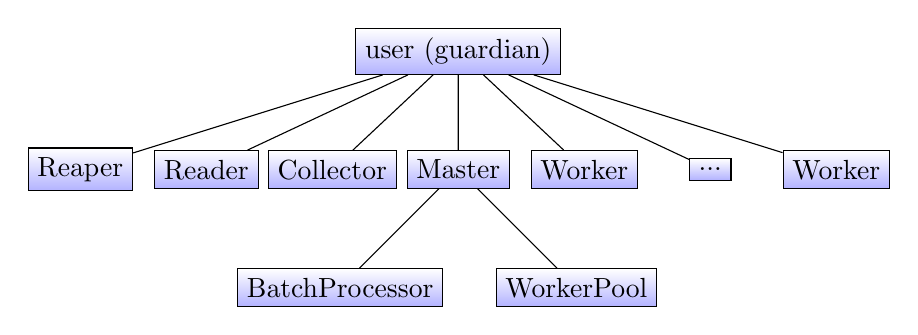
\begin{tikzpicture}[
			every node/.style = {shape=rectangle,
				draw, align=center,
				top color=white, bottom color=blue!30},
			level 1/.style={sibling distance=16mm},
			level 2/.style={sibling distance=30mm}]
			\node {user (guardian)}
				child { node {Reaper} }
				child { node {Reader} }
				child { node {Collector} }
				child { node {Master}
					child { node {BatchProcessor} }
					child { node {WorkerPool} }
				}
				child { node {Worker} }
				child { node {...} }
				child { node {Worker} };
		\end{tikzpicture}
	\end{figure}

	\begin{itemize}

		\item \textbf{Reaper}, \textbf{Reader} \& \textbf{Collector} mostly unchanged
		\item \textbf{Master}: Delegates worker registration messages to the worker pool and batches to the batch processor actors.
		\item \textbf{BatchProcessor}: Splits a batch into multiple work items for the worker actors and aggregates back the results
		\item \textbf{WorkerPool}: Routes and load balances the work items to the worker actors 

	\end{itemize}
\end{frame}

\begin{frame}
	\frametitle{Worker actor system}

	\begin{figure}[!h]
		\centering
		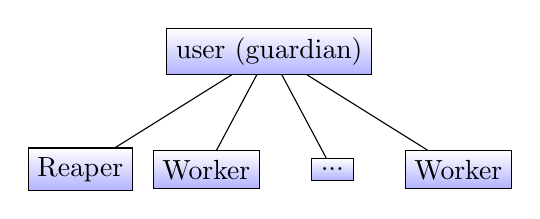
\begin{tikzpicture}[
			every node/.style = {shape=rectangle,
					draw, align=center,
					top color=white, bottom color=blue!30},
				level 1/.style={sibling distance=16mm}]
			\node {user (guardian)}
				child { node {Reaper} }
				child { node {Worker} }
				child { node {...} }
				child { node {Worker} };
		\end{tikzpicture}
	\end{figure}

	\begin{itemize}

		\item \textbf{Worker}s have two possible tasks:

		\begin{enumerate}

			\item Crack a set of hint hashes:

			\begin{itemize}

				\item \textbf{Input:} List of hint SHA256 hashes, possible characters, prefix

				\item \textbf{Output:} Hashtable of (hint SHA256 hash \textrightarrow \ missing character) for the cracked hints

			\end{itemize}

			\item Crack a password:

			\begin{itemize}

				\item \textbf{Input:} Password SHA256 hash, possible characters, length

				\item \textbf{Output:} Password SHA256 hash, password plaintext

			\end{itemize}

		\end{enumerate}

	\end{itemize}
\end{frame}

\begin{frame}[fragile]
	\frametitle{Hint cracking}

	Since each hint consists of all \texttt{PasswordChars} except one, it is fundamentally a permutation problem. Given the hash of a hint, we can crack it as follows:

	\begin{enumerate}
		\item Iterate over all permutations of \texttt{PasswordChars}.
		\item For each permutation, compute the SHA256 hash of all characters in the permutation except the last one.
		\item If the hash matches, we have cracked the hint!
	\end{enumerate}

	\pause

	E.g. in pseudocode:

	\begin{lstlisting}[language=Python]
def crack_hint(password_chars, hint_hash):
    for p in permutations(password_chars):
        candidate_hash = sha256(p[0:len(p)-2])
        if candidate_hash == hint_hash:
            # Return the missing character in the hint
            return p[len(p)-1]
    return None # Failed to crack hint
\end{lstlisting}
\end{frame}

\begin{frame}[fragile]
	\frametitle{Hint cracking (cont.)}

	However, since \textbf{all records in the CSV file} have the same \texttt{PasswordChars}, we do \emph{a lot} of redundant work if we apply the above algorithm for each single hint. \vspace{5mm}

	Instead, we can \textbf{simultaneously} crack many hint hashes in one iteration, by building a hashtable of hint hashes and checking whether the hash is in the hashtable. \vspace{5mm}

	\pause

	E.g. in pseudocode:

	\begin{lstlisting}[language=Python]
def crack_hints(password_chars, records):
    hint_hashes = set(h for h in r.hint_hashes for r in records)
    cracked_hint_hashes = dict()

    for p in permutations(password_chars):
        candidate_hash = sha256(p[0:len(p)-2])
        if candidate_hash in hint_hashes:
            # Store the missing character in the hint
            cracked_hint_hashes[candidate_hash] = p[len(p)-1]

    return cracked_hint_hashes
\end{lstlisting}

\end{frame}

\begin{frame}
	\frametitle{Distributing hint cracking}

	In order to efficiently parallelize and distribute the hint cracking, we need to figure a way to execute the process with many workers. This is done as follows:

	\begin{enumerate}

		\item The \textbf{BatchProcessor} partitions the hint cracking process evenly, using two-character prefixes of \texttt{PasswordChars}.

		\begin{itemize}

			\item E.g. if \texttt{PasswordChars} is ABCDEFGHIJK, the prefixes are AB, AC, AD, ..., JH, JI, JK.

			\item The first work item will iterate over the permutations of the form AB***********, the second on AC***********, etc..

			\item \textrightarrow 110 work items are created.

		\end{itemize}

		\pause

		\item Work items are routed and load balanced among the worker actors by the \textbf{WorkerPool}.

		\item The \textbf{Worker}s execute the hint cracking algorithm over their partition of the process and return the cracked hints to the \textbf{BatchProcessor}

		\item The \textbf{BatchProcessor} receives back and aggregates the results.

	\end{enumerate}

\end{frame}

\begin{frame}[fragile]
	\frametitle{Password cracking}

	Once all hints are cracked, cracking the passwords is straightforward as a combination problem. Given the hash of a password, we can crack it as follows:

	\begin{enumerate}

		\item Iterate over all combinations of the remaining \texttt{PasswordChars} after solving for the hints.
		\item For each combination, compute the SHA256 hash of all characters in the combination.
		\item If the hash matches, we have cracked the password!

	\end{enumerate}

	\pause

	E.g. in pseudocode:

	\begin{lstlisting}[language=Python]
def crack_password(remaining_password_chars, password_hash, password_length):
    for c in combinations(remaining_password_chars, password_length):
        candidate_hash = sha256(c)
        if candidate_hash == password_hash:
            # Return the password plaintext
            return c
    return None # Failed to crack password
\end{lstlisting}

\end{frame}

\begin{frame}
	\frametitle{Distributing password cracking}

	Distributing the password cracking is straightforward: One work item is created for every password to crack.

	\begin{enumerate}

		\item Once the \textbf{BatchProcessor} has received all cracked hints for a record in the batch, it generates a new work item to crack the password.

		\item Work items are routed and load balanced among the worker actors by the \textbf{WorkerPool}.

		\item The \textbf{Worker}s execute the password cracking algorithm and return the cracked password to the \textbf{BatchProcessor}

		\item The \textbf{BatchProcessor} gives the password plaintext to the \textbf{Collector} to be printed later.

		\item Once all passwords are cracked, the \textbf{BatchProcessor} sends a message to the \textbf{Master}, which causes a new batch to be read.

	\end{enumerate}

\end{frame}

\begin{frame}
	\frametitle{Optimization}

	While we are doing parallel and distributed computation, \textbf{implementing the algorithms efficiently} is still very important for overall performance!

	\begin{itemize}

		\item Efficient permutation iteration is not trivial, but there are algorithms for it:

		\begin{itemize}

			\item "Countdown QuickPerm Algorithm" (by Phillip Paul Fuchs)

		\end{itemize}

		\pause

		\item Avoid common Java performance pitfalls. E.g.:

		\begin{itemize}

			\item Avoid concatatenating \texttt{String}s (causes a copy)

			\item Avoid repeatedly calling \texttt{String.getBytes()} (causes a copy)

			\item \texttt{MessageDigest} instances can be reused

			\item ...

		\end{itemize}
	\end{itemize}
\end{frame}

\begin{frame}
	\frametitle{Results}

	\begin{itemize}

		\item \textbf{Good performance:} Even when running on a single node (typical laptop), the full process is very fast (e.g. <20 seconds with 4 workers).

		\item \textbf{Good scalability:} The master does few work, and the workload is split on many work items, so that it can be efficiently distributed over a moderately-sized cluster.

	\end{itemize}

\end{frame}

\begin{frame}
	\frametitle{Weak points}

	\begin{enumerate}

		\item We are not resistant to message loss or workers disconnections.
		\begin{itemize}
			\item \textbf{Solution:} Add disconnection and retry logic.
		\end{itemize}

		\item We are not resistant to invalid / uncrackable inputs.

		\begin{itemize}
			\item \textbf{Solution:} Add more validation logic.
		\end{itemize}

		\item The single \texttt{BatchProcessor} on the master system is relatively light, but it could become a bottleneck if the data set and the cluster becomes large.

		\begin{itemize}

			\item \textbf{Possible solution:} Process multiple batches simultaneously, with multiple \texttt{BatchProcessor}s.

		\end{itemize}

	\end{enumerate}

	\pause

	None of those problems are fundamental, and can be solved at the expense of somewhat increased effort and code complexity.

\end{frame}


\end{document}

